\documentclass[aps,prb,onecolumn,notitlepage,showpacs,floatfix,superscriptaddress]{revtex4-1}
\usepackage{dcolumn}
\usepackage{tabularx}
\usepackage{bm}
\usepackage{soul}
\usepackage{amsmath,amssymb,graphicx}
\usepackage[colorlinks=true,citecolor=blue,urlcolor=blue,linkcolor=blue]{hyperref}
\usepackage{environ}

\NewEnviron{eqnsplit}{%
\begin{equation}
\begin{split}
  \BODY
\end{split}
\end{equation}
}

\newcommand{\mrm}[1]{\mathrm{#1}}
\newcommand{\ang}{\mathrm{\AA}}
\newcommand{\bmp}{{\bm p}}
\newcommand{\Heff}{{\bm H}_\mathrm{eff}}
\newcommand{\heff}{{\bm h}_\mathrm{eff}}
\newcommand{\heffx}{{\bm h}^{x}_\mathrm{eff}}
\newcommand{\heffy}{{\bm h}^{y}_\mathrm{eff}}
\newcommand{\heffz}{{\bm h}^{z}_\mathrm{eff}}
\newcommand{\sint}{\sin\theta}
\newcommand{\cost}{\cos\theta}
\newcommand{\sinp}{\sin \phi}
\newcommand{\cosp}{ \cos\phi}

\newcommand{\sx}{\sin\theta \cos\phi}
\newcommand{\sy}{\sin\theta \sin\phi}
\newcommand{\sz}{\cos\theta}

\newcommand{\fe}{ \mathcal{F}}

\bibliographystyle{apsrev4-1}

%%%%%%%%%%%%%%%%%%%%%%%%%%%%%%%%%%%%%%%%%%%%%%%%
\begin{document}
\title{Notes: Ferromagnetic Resonance (FMR)}

\author{Avinash Rustagi}
\email{arustag@purdue.edu}
%
\date{\today}
%%%%%%%%%%%%%%%%%%%%%%%%%%%%%%%%%%%%%%%%%%%%%%%%

\maketitle
%
Ferromagnets (FM) are magnetically ordered materials characterized by the a spontaneous magnetization. Typically, FM have domains where the magnetization is uniform however a simple FM may have randomly oriented domains. In the macrospin description, a FM has a single domain. 

Magnetization i.e. magnetic moment per unit volume is proportional to the angular momentum and the coefficient relating the two is the gyromagnetic ratio. It is well known that the rate of change of angular momentum is equal to the torque. Thus in presence of an effective magnetic field, the dynamics of the magnetization can be simply described by the equation of motion
\begin{equation}
\dfrac{d{\bm M}}{dt} = - \gamma ({\bm M} \times {\bm H}_\mrm{eff}) \qquad \gamma : \text{Gyromagnetic Ratio}
\end{equation}
The first observation from this equation is that the magnitude of magnetization remains constant
\begin{equation}
{\bm M} \cdot \dfrac{d{\bm M}}{dt} = 0 \Rightarrow \vert {\bm M} \vert = \text{constant} \equiv M_s
\end{equation}
Thus, only the orientation of the magnetization vector changes under the effective magnetic field. For describing such a system, it is particularly convenient to move to spherical coordinates characterized by $(\hat{M},\hat{\theta},\hat{\phi})$ where the relation to cartesian coordinates is
\begin{eqnsplit}
\hat{M} &= \sint \cosp \,\hat{x} + \sint \sinp \,\hat{y} + \cost \,\hat{z} \\
\hat{\theta} &= \cost \cosp  \,\hat{x} + \cost \sinp \,\hat{y} - \sint \,\hat{z} \\
\hat{\phi} &=-\sinp \, \hat{x} + \cosp \,\hat{y} 
\end{eqnsplit}
\begin{figure}[hbtp]
\centering
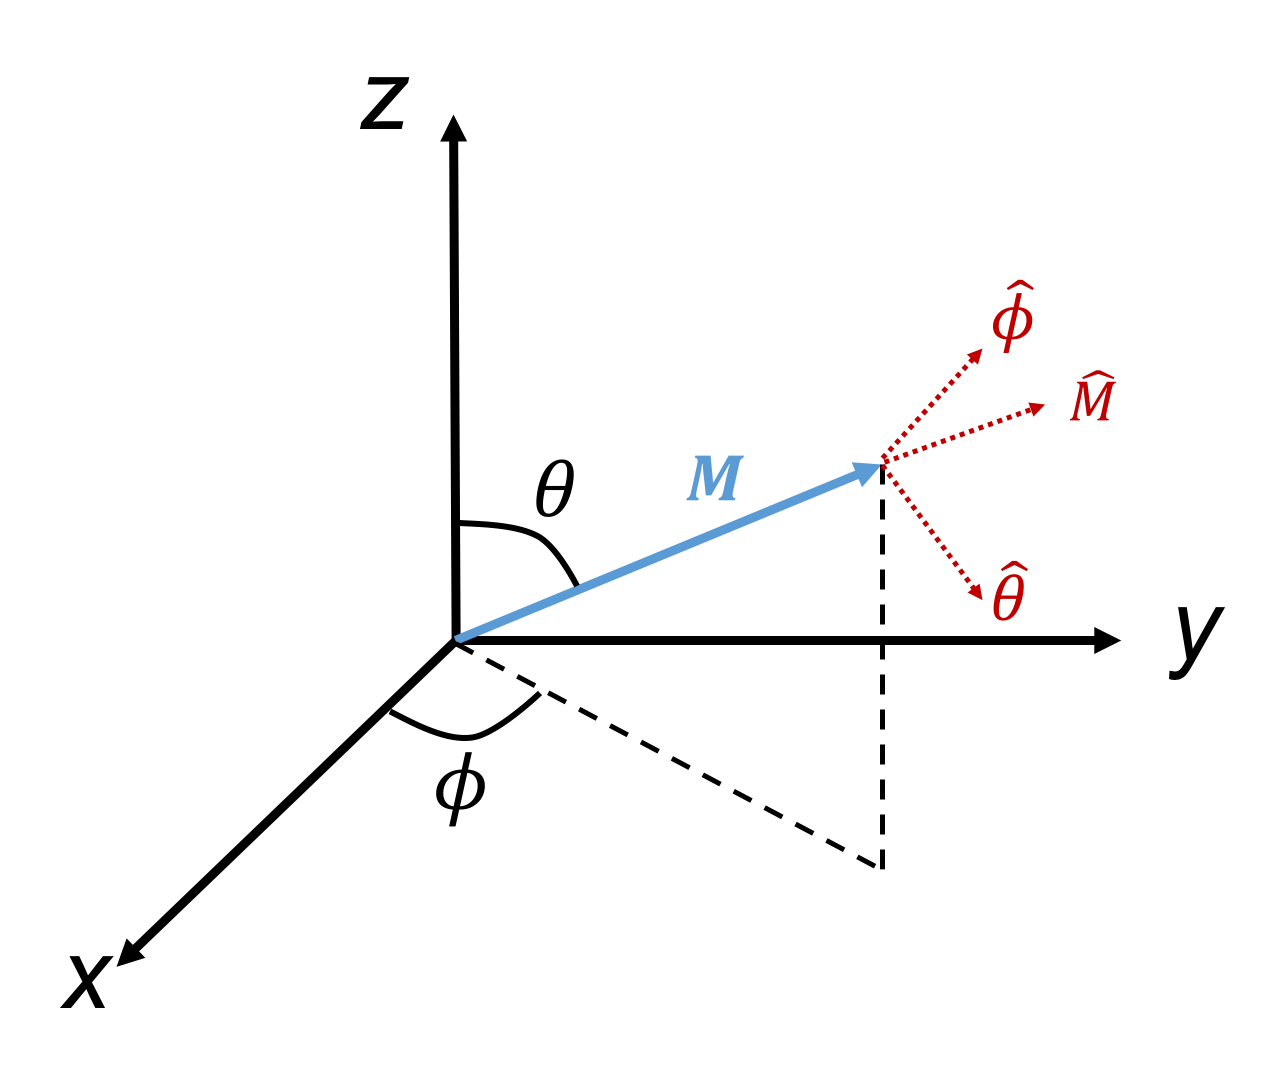
\includegraphics[scale=0.4]{MPolarCoordinates.png}
\caption{Coordinate System}
\end{figure}
The magnetic field in this coordinate system is
\begin{eqnsplit}
{\bm H} &= H_M \hat{M} + H_\theta \hat{\theta} + H_\phi \hat{\phi} \\
H_M &=  \sint \cosp H_x + \sint \sinp H_y+ \cost H_z \\
H_{\theta} &= \cost \cosp  H_x + \cost \sinp H_y - \sint H_z\\
H_{\phi} &=-\sinp H_x + \cosp H_y
\end{eqnsplit}
Looking the the equation of motion for the z-component
\begin{equation}
\begin{split}
& \dfrac{d M_z}{dt} = -\gamma (M_x H_y - M_y H_x) \\
\Rightarrow & -\sint \dfrac{d\theta}{dt} = -\gamma \sint (-\sinp H_x + \cosp H_y) \\
\Rightarrow & \dfrac{d\theta}{dt} = \gamma H_\phi
\end{split}
\end{equation}
and from the equation of motion for the x-component
\begin{equation}
\begin{split}
& \dfrac{d M_x}{dt} = -\gamma (M_y H_z - M_z H_y) \\
\Rightarrow & -\sint \sinp \dfrac{d\phi}{dt} +\cost \cosp \dfrac{d\theta}{dt} = -\gamma  (\sint \sinp H_z - \cost H_y) \\
\Rightarrow & \sint \dfrac{d\phi}{dt} = -\gamma H_\theta
\end{split}
\end{equation}

The effective magnetic field governing the magnetization dynamics can be derived from the free energy
\begin{equation}
{\bm H}_\mrm{eff} = -\dfrac{1}{M_s} \dfrac{d\fe}{d{\hat{M}}}
\end{equation}
and the free energy landscape of the magnet has contributions from the external field, the effective anisotropy (anisotropy + demagnetization), random noise. 

Given free energy density $\fe$, the equilibrium orientation of the magnetization can be determined by minimizing the free energy density.
\begin{equation}
\dfrac{d\fe}{d\theta} = 0 \qquad \dfrac{d\fe}{d\phi}=0 \qquad \Rightarrow \{\theta_0,\phi_0\}
\end{equation}
\begin{figure}[hbtp]
\centering
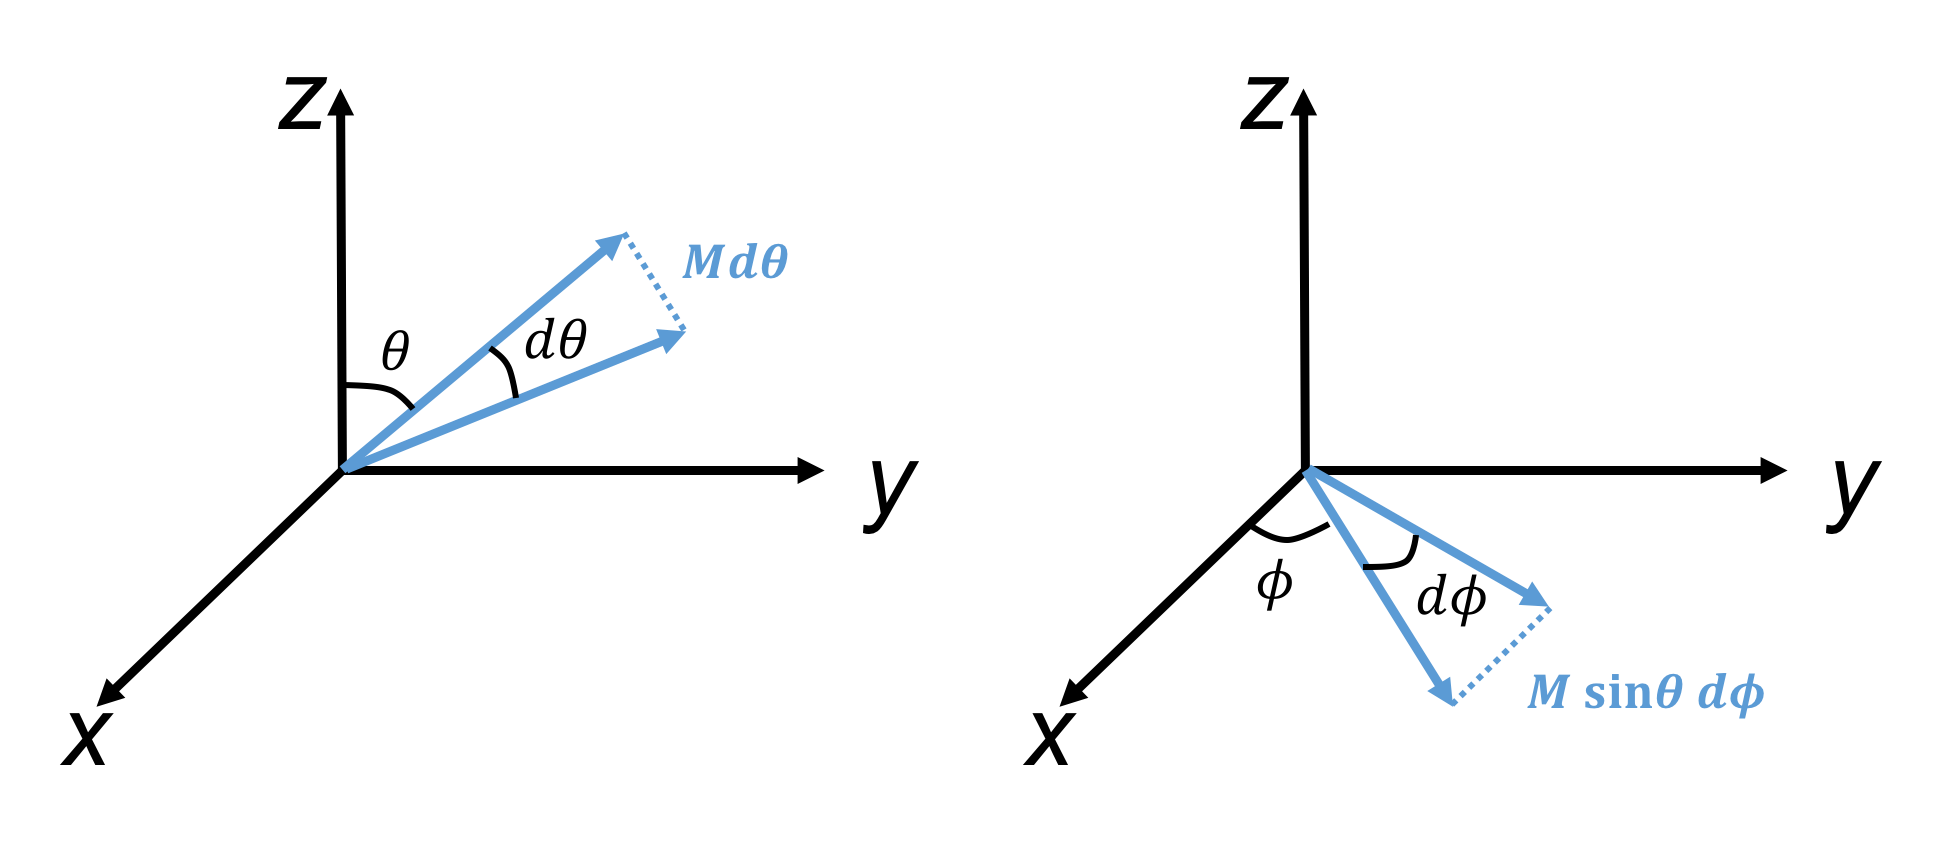
\includegraphics[scale=0.4]{MChange.png}
\caption{Magnetization changes due to small angle deviations.}
\end{figure}
If the magnetization deviates from the equilibrium position due to the action of the magnetic field components, the change in free energy can be related to the field components
\begin{equation}
\begin{split}
&d\fe=-M_s d\theta \, H_\theta  \qquad \Rightarrow \fe_\theta = \dfrac{d\fe}{d\theta} = -M_s H_\theta \\
&d\fe=-M_s \sint d\phi \, H_\phi  \qquad \Rightarrow \fe_\phi = \dfrac{d\fe}{d\phi} = -M_s \sint \, H_\phi \\
\end{split}
\end{equation}
Thus, the equation of motion of the angular coordinates can be expressed in terms of the free energy derivatives
\begin{equation}
\begin{split}
&\dfrac{d\theta}{dt} = \gamma H_\phi = -\gamma \dfrac{\fe_\phi}{M_s \sint} \\
&\sint \dfrac{d\phi}{dt} = -\gamma H_\theta = \gamma \dfrac{\fe_\theta}{M_s}
\end{split}
\end{equation}
Assuming that the angular deviations from equilibrium are small $\delta\theta = \theta - \theta_0 \ll \theta_0$ and $\delta\phi = \phi - \phi_0 \ll \phi_0$, we can Taylor expand the free energy in terms of derivatives
\begin{equation}
\fe_\theta = \fe_{\theta \theta} \delta\theta +  \fe_{\theta \phi} \delta\phi \qquad  \fe_\phi = \fe_{\phi \theta} \delta\theta +  \fe_{\phi \phi} \delta\phi
\end{equation}
where the double derivatives $\fe_{\theta \theta}, \fe_{\theta \phi},\fe_{\phi \theta}, \fe_{\phi \phi}$ are evaluated at the equilibrium. Therefore the equations of motion in the linearized regime of the small angular deviations are
\begin{equation}
\begin{split}
&\dfrac{d\delta \theta}{dt} = -\dfrac{\gamma}{M_s \sint} \left[ \fe_{\phi \theta} \delta\theta +  \fe_{\phi \phi} \delta\phi \right] \\
\sint_0 &\dfrac{d\delta\phi}{dt}  =  \dfrac{\gamma}{M_s} \left[ \fe_{\theta \theta} \delta\theta +  \fe_{\theta \phi} \delta\phi  \right]
\end{split}
\end{equation}
Harmonic solutions $\delta\theta \sim e^{-i\omega t}, \delta\phi \sim e^{-i\omega t}$ exist if
\begin{equation}
\fe_{\theta \theta} \fe_{\phi \phi}- \fe_{\phi \theta} \fe_{\theta \phi} + \dfrac{\omega^2}{\gamma^2} M_s^2 \sint_0^2 =0
\end{equation}
which provides the resonance frequency
\begin{equation}
\omega_\mrm{res} = \dfrac{\gamma}{M_s \sint_0} \sqrt{\fe_{\theta \theta} \fe_{\phi \phi}-  \fe_{\theta \phi}\fe_{\phi \theta}}
\end{equation}

\section{Example: Magnetic thin film with in-plane magnetization}
Here we consider a magnetic thin film with in-plane equilibrium magnetization. The system has a uniaxial anisotropy which makes the magnetization align in the equilibrium direction. It also has a perpendicular magnetic anisotropy which includes both the demagnetization field and the interface field due to the substrate.
\begin{figure}[hbtp]
\centering
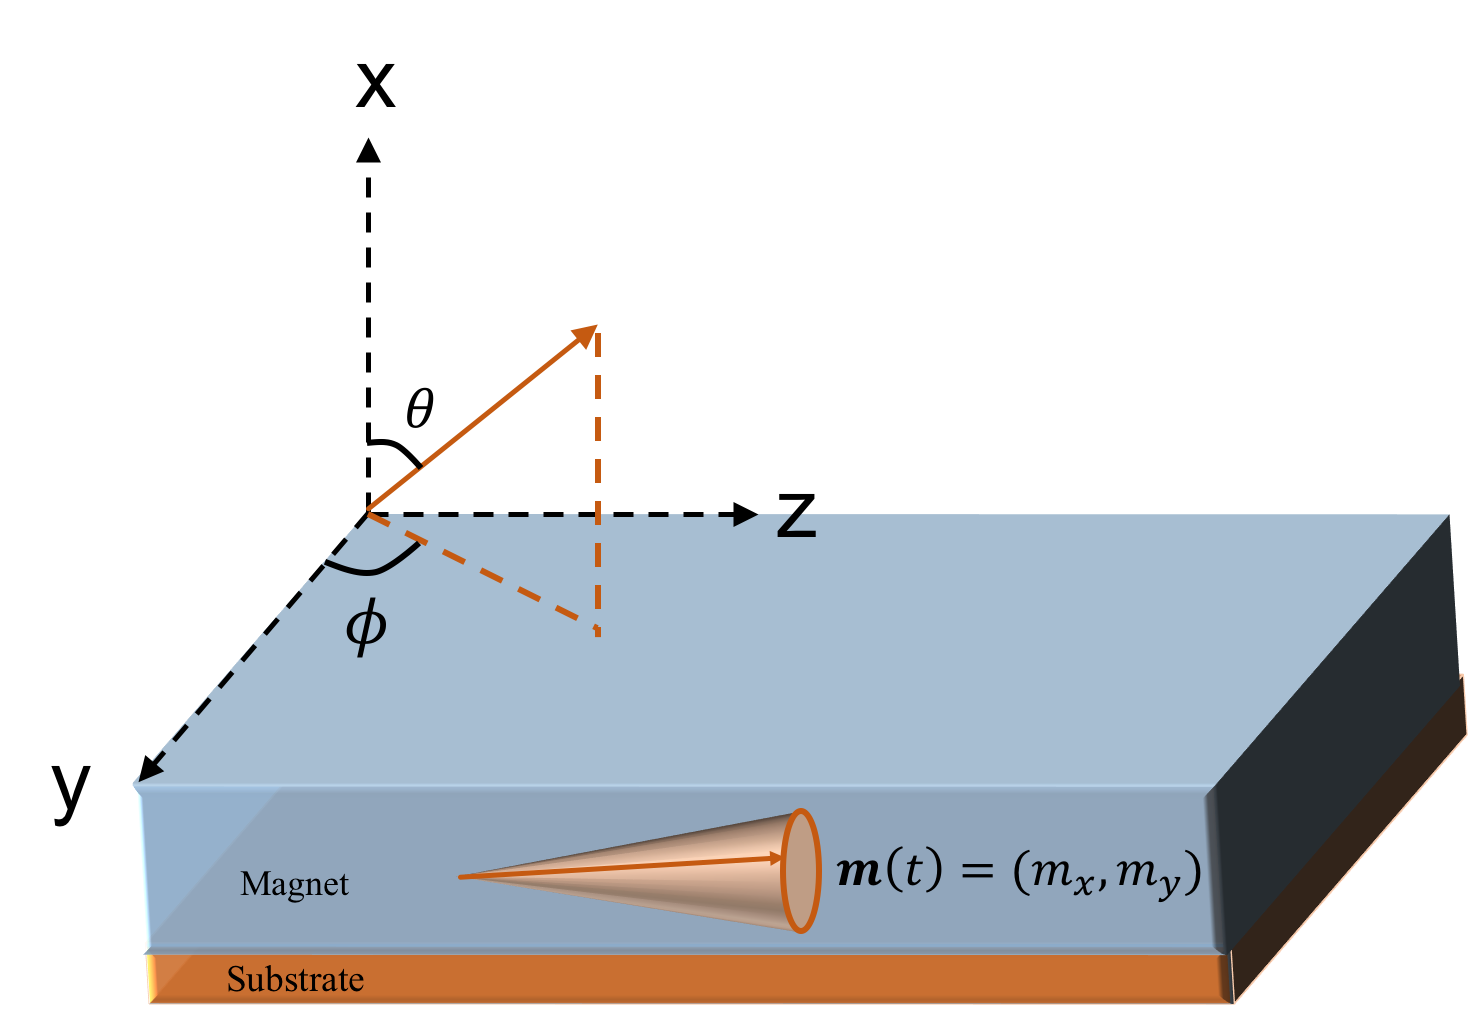
\includegraphics[scale=0.4]{FMR_InPlaneMagnet.png}
\caption{Schematic of the in-plane magnet.}
\end{figure}
The general free energy density for such a ferromagnet with in-plane equilibrium magnetization has the following pieces (in terms of the unit magnetization vector $\hat{M}=[m_x,m_y,m_z]$):
\begin{itemize}
\item Zeeman term due to external applied field (along z-axis): $\fe_z = - M_s \, \hat{M}\cdot {\bm H} = - M_s H m_z$
\item Uniaxial anisotropy which prefers orientation along the z-axis: $\fe_u = - K m_z^2$
\item Demagnetization: $\fe_d =  - \dfrac{ M_s}{2} \, \hat{M}\cdot {\bm H}_d$ where the demagnetizing field ${\bm H}_d = - M_s \overline{\overline{\bm N}} \hat{M}$. $\overline{\overline{\bm N}}$ is the demagnetization tensor which for the considered thin film geometry has only non-zero $N_{xx} = 4\pi$. Therefore $\fe_d =   2\pi M_s^2 \, m_x^2$.
\item Interface anisotropy: The presence of the interface between the magnet and substrate provides an additional anisotropy due the difference in the material environment in the magnet and substrate. This effect is particularly significant in thin films as the anisotropy affecting the entire film thickness is important to the orientation of magnetization. In a simplest of explanations, one expects that the charges/ions close to the interface will want the magnetization to orient perpendicular to the interface due to spin-orbit interaction (angular momentum wants spins to align them along due to ${\bm L}\cdot{\bm S}$) and crystal field effects. The free energy is of the form $\fe_i = - \dfrac{K_i}{t_\mrm{fm}} m_x^2 \equiv - K_t m_x^2$. This is a very significant term as it explains the VCMA (Voltage Controlled Magnetic Anisotropy) effect.
\end{itemize}

The combination of the demagnetization energy and the interface anisotropy is referred to as the perpendicular magnetic anisotropy (PMA). Thus the total free energy density for the system is
\begin{equation}
\begin{split}
\fe  &=  - M_s H m_z - K m_z^2 + 2\pi M_s^2 \, m_x^2 - K_t m_x^2 \\
&=  - M_s H m_z - K m_z^2 +\dfrac{M_s}{2} \left[  4\pi M_s - \dfrac{2 K_t}{M_s} \right] m_x^2 \\
&=  - M_s H m_z - K m_z^2 +\dfrac{M_s}{2} H_{\perp} m_x^2 \\
\end{split}
\end{equation}
where the PMA field is $H_\perp = \left[  4\pi M_s - \dfrac{2 K_t}{M_s} \right]$. From the free energy form, we can physically infer that for positive $H_\perp$, the magnet will preferably orient along the z-axis. However for negative $H_\perp$, there will be a critical external field below which the magnet will prefer to orient along the x-axis. This control on the orientation of the magnetization is provided by the VCMA effect. In terms of polar coordinates, the free energy is
\begin{equation}
\begin{split}
\fe  &=  - M_s H m_z - K m_z^2 +\dfrac{M_s}{2} H_{\perp} m_x^2 \\
&=  - M_s H \sint \sinp - K \sin^2 \theta \sin^2 \phi +\dfrac{M_s}{2} H_{\perp} \cos^2 \theta \\
\end{split}
\end{equation}
The equilibrium orientation of the magnet is determined by minimizing the free energy of the magnet
\begin{equation}
\begin{split}
\fe_\theta  &=  - M_s H \cost \sinp - 2 K \sint \cost \sin^2 \phi -M_s H_{\perp} \sint \cost \equiv 0 \\
\fe_\phi  &=  - M_s H \sint \cosp - 2 K \sin^2 \theta \sinp \cosp \equiv 0 \\
\end{split}
\end{equation}
From the above minimization conditions, we can infer that the angle $\phi_0 = \pi/2$. This is so because VCMA can shift orientation of the magnetization in the x-z plane. Thus, the condition for $\theta$ is given by
\begin{equation}
- M_s \cost \left[ H   + \left(H_k+ H_{\perp}\right) \sint \right] = 0
\end{equation}
where $H_k = 2K/M_s$ - the uniaxial anisotropy field. This provides two possible solutions: $\theta= \pi/2$ or $\sint = - H /\left(H_k+ H_{\perp}\right)$. We note that the polar angle $\theta \in [0,\pi]$. Thus 
\begin{itemize}
\item For $H_k+ H_{\perp} > 0$, $\theta = \pi/2$. 
\item For $H_k+ H_{\perp} < 0$ and $H < \vert H_k+ H_{\perp} \vert $, $\sint = H /\vert H_k+ H_{\perp}\vert$.
\item For $H_k+ H_{\perp} < 0$ and $H > \vert H_k+ H_{\perp} \vert $, $\theta = \pi/2$.
\end{itemize}

\subsection*{\underline{Case 1:  $\theta=\pi/2$ and $\phi=\pi/2$}}
For evaluating the FMR frequency, we need to calculate the second derivatives of the free energy density at the equilibrium.
\begin{equation}
\begin{split}
\fe_{\theta \theta}  &=  M_s H \sint \sinp - 2 K \cos 2\theta \sin^2 \phi -M_s H_{\perp} \cos 2\theta = M_s H  + 2 K  + M_s H_{\perp}  \\
\fe_{\phi \theta}  &=  - M_s H \cost \cosp - 2 K \sin 2 \theta \sinp \cosp = 0  \equiv \fe_{\theta \phi} \\
\fe_{\phi \phi}  &=   M_s H \sint \sinp - 2 K \sin^2 \theta \cos 2\phi = M_s H  + 2 K 
\end{split}
\end{equation}
Therefore
\begin{equation}
\begin{split}
\omega_\mrm{res} &=  \dfrac{\gamma}{M_s \sint_0} \sqrt{\fe_{\theta \theta} \fe_{\phi \phi}-  \fe_{\theta \phi}\fe_{\phi \theta}}\\
&= \dfrac{\gamma}{M_s} \sqrt{\left(M_s H  + 2 K  + M_s H_{\perp} \right) \left( M_s H  + 2 K  \right) } \\
&=\gamma \sqrt{\left( H  + \dfrac{2 K}{M_s}  +  H_{\perp} \right) \left( H  + \dfrac{2 K}{M_s} \right) } \\
&=\gamma \sqrt{\left( H  + H_k  +  H_{\perp} \right) \left( H  + H_k \right) } \\
\end{split}
\end{equation}

\subsection*{\underline{Case 2: $H_k+ H_{\perp} = - \vert H_k+ H_{\perp} \vert<0$; $\sint=H /\vert H_k+ H_{\perp}\vert$ and $\phi=\pi/2$}}
For evaluating the FMR frequency, we need to calculate the second derivatives of the free energy density at the equilibrium.
\begin{equation}
\begin{split}
\fe_{\theta \theta}  &=  M_s H \sint \sinp - 2 K \cos 2\theta \sin^2 \phi -M_s H_{\perp} \cos 2\theta  \\
&=  \dfrac{M_s H^2 }{\vert H_k+ H_{\perp}\vert} - M_s \left(H_k+H_\perp\right) \left( 1- \dfrac{2H^2}{(H_k+ H_{\perp})^2}\right) \\
&=  \dfrac{M_s H^2 }{\vert H_k+ H_{\perp}\vert} - M_s \left(H_k+H_\perp\right) + \dfrac{2M_s H^2}{(H_k+ H_{\perp})} \\
&=  M_s \vert H_k+H_\perp \vert - \dfrac{M_s H^2}{\vert H_k+ H_{\perp} \vert} \\
\fe_{\phi \theta}  &=  - M_s H \cost \cosp - 2 K \sin 2 \theta \sinp \cosp = 0  \equiv \fe_{\theta \phi} \\
\fe_{\phi \phi}  &=   M_s H \sint \sinp - 2 K \sin^2 \theta \cos 2\phi \\
&=  \dfrac{M_s H^2}{\vert H_k+ H_{\perp}\vert}  + 2 K \dfrac{H^2}{(H_k+ H_{\perp})^2}\\
&=  \dfrac{M_s H^2}{\vert H_k+ H_{\perp}\vert} \left(1  +  \dfrac{H_k}{\vert H_k+ H_{\perp}\vert} \right)
\end{split}
\end{equation}
Therefore
\begin{equation}
\begin{split}
\omega_\mrm{res} &=  \dfrac{\gamma}{M_s \sint_0} \sqrt{\fe_{\theta \theta} \fe_{\phi \phi}-  \fe_{\theta \phi}\fe_{\phi \theta}}\\
&= \dfrac{\gamma}{M_s \sint} \sqrt{ \dfrac{M_s H^2}{\vert H_k+ H_{\perp}\vert} \left(1  +  \dfrac{H_k}{\vert H_k+ H_{\perp}\vert} \right)\left( M_s \vert H_k+H_\perp \vert - \dfrac{M_s H^2}{\vert H_k+ H_{\perp} \vert} \right)} \\
&= \gamma \sqrt{ \left(1  +  \dfrac{H_k}{\vert H_k+ H_{\perp}\vert} \right)\left[  ( H_k+H_\perp )^2 - H^2 \right]} \\
\end{split}
\end{equation}

To summarize, the FMR frequency in different regimes are:
\begin{itemize}
\item For $H_k+ H_{\perp} > 0$, $\theta = \pi/2$:\\
 $$\omega_\mrm{res}=\gamma \sqrt{\left( H  + H_k  +  H_{\perp} \right) \left( H  + H_k \right) }$$
\item For $H_k+ H_{\perp} < 0$ and $H < \vert H_k+ H_{\perp} \vert $, $\sint = H /\vert H_k+ H_{\perp}\vert$:\\
$$\omega_\mrm{res}=\gamma \sqrt{ \left(1  +  \dfrac{H_k}{\vert H_k+ H_{\perp}\vert} \right)\left[  ( H_k+H_\perp )^2 - H^2 \right]} $$
\item For $H_k+ H_{\perp} < 0$ and $H > \vert H_k+ H_{\perp} \vert $, $\theta = \pi/2$: \\
$$\omega_\mrm{res}=\gamma \sqrt{\left( H  + H_k  +  H_{\perp} \right) \left( H  + H_k \right) }$$
\end{itemize}

\begin{table}[h]
\caption{\label{summary} Summarizing the FMR frequency expressions: }
\begin{ruledtabular}
\begin{tabular}{lr}
Condition & FMR Resonance Frequency \\
\hline
\\
$H_k+ H_{\perp} > 0$	  & $\omega_\mrm{res}=\gamma \sqrt{\left( H  + H_k  +  H_{\perp} \right) \left( H  + H_k \right) }$ \\
\\
$H_k+ H_{\perp} < 0$ and $H < \vert H_k+ H_{\perp} \vert $, $\sint = H /\vert H_k+ H_{\perp}\vert$ & $\omega_\mrm{res}=\gamma \sqrt{ \left(1  +  \dfrac{H_k}{\vert H_k+ H_{\perp}\vert} \right)\left[  ( H_k+H_\perp )^2 - H^2 \right]} $\\
\\
$H_k+ H_{\perp} < 0$ and $H > \vert H_k+ H_{\perp} \vert $, $\theta = \pi/2$ & $\omega_\mrm{res}=\gamma \sqrt{\left( H  + H_k  +  H_{\perp} \right) \left( H  + H_k \right) }$ \\
\end{tabular}
\end{ruledtabular}
\end{table}

\end{document}
